\subsection{Проектирование и разработка клиентской части программного средства}
\label{sec:design:client}

Задачи клиентской части приложения включают отображение пользовательского интерфейса и обработку действий пользователя. Типичными этапами его проектирования являются следующие~\cite[с.~78]{application_architecture_guide}:

\begin{itemize}
	\item Идентификация типа клиентской части приложения, которое удовлетворяет установленным требованиям. Осуществление данного этапа осуществлено в подразделе~\ref{sec:design:architecture}.
	\item Выбор технологии пользовательского интерфейса. Осуществляется на основе анализа требуемой для реализации функциональности.
	\item Проектирование UI. Хорошей практикой является реализация модульности, а также принципа разделения ответственности компонентов.
	\item Определение стратегии и протоколов обмена информации между уровнями. Поскольку рассматриваемый уровень является самым верхним, а его протоколы связи с серверной частью приложения были рассмотрены в пункте~\ref{sec:design:server:protocols}, то данный вопрос считается решенным и рассматриваться не будет.
\end{itemize}

Ранее был проведен анализ и осуществлен выбор целевой платформы для реализации клиентской части приложения, был выбран основной язык программирования. 
Однако, существует огромное число специализированных технологий и фреймворков по созданию пользовательских интерфейсов. 
Представляется целесообразным провести уточнение средств разработки.

\subsubsection{} Уточнение выбора технологий программирования
\label{sec:design:client:technologies}

Язык программирования \csharp является языком общего назначения. Он является строготипизированным, то есть компилятор проверяет соответствие типов при работе
с данными. Код, написанный на \csharp может быть скомпилирован компилятором MSVC от компании Microsoft. Для того, чтобы программная среда Visual Studio поддерживала
программы на \csharp необходимо воспользоваться пакетным менеджером Visual Studio Installer, в котором нужно выбрать пакет инструментов для разработки под платформу .NET.
После установки инструментов в среде можно создать проект, с целевой платформой .NET, где и будут использоваться установленные ранее инструменты. Все работает по умолчанию и
программисту не нужно тратить свое время на дополнительную настройку.

При разработке настольных приложений на платформе .NET есть два основных подхода: WinForms и WPF. Рассмотрим каждый из них подробнее.

WinForms - первоначальный подход к высокоуровневому проектированию пользовательского интерфейса на платформе .NET. До их появления, единственным вариантом для программиста было использование WinApi, которое
является крайне не удобным с точки зрения разработки комплексных решения для пользовательского интерфейса. Главным минусом WinApi является то, что он не является кроссплатформенным, так как доступен
только на платформе с операционной системой Windows, что и следует из названия. Для решения этой проблемы инженеры компании Microsoft и придумали слой абстракций для разработки пользовательского
интерфейса, который получил название WinForms. Ключевой особенностью является то, что разработанный пользовательский интерфейс является кроссплатформенным, то есть может работать, например, под
операционной системой Linux. Разработка интерфейса происходит с помощью перетягивания элементов управления на окно дизайнера интерфейса. Такой подход позволяет быстро реализовать самые сложные интерфейсы
за счет того, что больше не нужно тратить время на поиск нужных функций WinApi, к тому же его не нужно переписывать в случае, если приложение разрабатывается под несколько платформ. Не смотря
на удобство в использовании, разработанный с помощью WinForms интерфейс имеет ряд недостатков, которые сложно устранить штатными средствами, а именно: 

\begin{itemize}
	\item Отсутствие глубокой кастомизации внешнего вида элементов управления. Программист может выбрать один из нескольких уже готовых пресетов, а в случае если нужного пресета нет, то необходимо прибегать к WinApi, из-за чего теряется кроссплатформенность.
	\item В подавляющем числе случаев интерфейс не будет является адаптивным по отношению к размерам окна. Это снижает удобство использования для конечных пользователей.
	\item Использование обработчиков событий является устаревшим подходом. Такой подход сильно связывает пользовательский интерфейс и классы-контроллеры, что ухудшает расширяемость и снижает продуктивность разработки.
\end{itemize}

Несмотря на все недостатки, WinForms были популярны достаточно долгое время, благодаря низкому порогу вхождения и простоте проектирования. Инженеры Microsoft проанализировали недостатки WinForms и
сделали новый пакет инструментов, устраняющий все недостатки, упомянутые выше. Он получил название WPF -- Windows Presentation Foundation.

WPF представляет из себя дизайнер, который поддерживает привязки к данным, разработку адаптивного интерфейса, а также глубокую систему стилей, со своими видами наследования, а также обработчиками
в контексте пользовательского интерфейса, которые называются триггерами. Рассмотрим основные возможности платформы WPF.

Представления, как обособленные сущности, являются полностью независимыми от какого-либо контекста и могут обрабатывать действия пользователя никого не уведомляя. Для этих целей 
используются триггеры -- специальные процедуры, которые срабатывают в заданном программистом случае и чаще всего выполняют примитивные задачи. Например скрытие списка, если он пуст. 
Триггер должен проверять содержимое элемента управления (ItemsSource) и если количество (Count) элементов равно нулю, то видимомость элемента управления (Visibility) устанавливается в false.
Это лишь один из многих примеров использования триггеров, с их помощью можно автоматизировать множество задач без необходимости написания кода обработчиков.

При разработке формата представлений инженеры вдохновлялись \linebreak HTML и CSS, типичное представление содержит информацию о расположении элементов управления в формате XAML.
XAML очень похож на HTML, его главной особенностью является то, что он расширяемый, то есть программист может писать свои расширения разметки, которые можно будет использовать в разработке.
Одной из сильнейших сторон WPF по сравнению с WinForms является система стилей. Она похожа на CSS из мира веб-разработки. Каждый элемент управления имеет свой набор атрибутов, таких как
видимость, цвет фона, шрифт, размер шрифта и так далее. Все это можно оформить в один стиль, дать ему имя, которое будет является ключом и всем похожим элементам управления присваивать ключ стиля. 
Таким образом все одинаковые элементы управления будут иметь одинаковые стили, которые в случае чего можно будет поменять только в одном месте. Стоит также отметить, что
все стили поддерживают механизм наследования, то есть при желании разработчик может добавить новый атрибут к стилю, при этом сохранив все значения атрибутов базового стиля, 
что особенно удобно когда нужно внести минимальные правки, но создавать стиль с нуля слишком накладно.

Еще одним существенным отличием WPF от WinForms является наличие шаблонных элементов управления и поддержка автогенерации интерфейса. В WinForms для генерации нужно было использовать
code-behind самой формы, что увеличивало уровень связности, а также приводило к большому количеству шаблонного кода, который не решал никакой бизнес-задачи. В WPF эту проблему решили,
позволив создавать шаблоны пользовательского интерфейса, причем шаблоны могут отличаться в зависимости от текущего типа данных, для которого генерируется интерфейс. Например, у программиста
есть три класса, которые реализуют один и тот же интерфейс и хранятся в списке как интерфейс класса, генератор UI может определять какой тип содержит каждый элемент из списка и
создавать требуемый формат для заполнения полей. Для этого используется концепт pattern-matching \cite{msdn_pattern_matching}.

Про привязку данных уже шла речь в разделе \ref{sec:design:tester:editor}, поэтому здесь пойдет речь про команды, как механизм реакции на действия пользователя.
Одним из главных недостатков WinForms являлся механизм событий, который жестко связывал конкретный элемент управления и код обработчика. Команды в свою очередь призваны 
предоставить требуемый уровень абстракций, позволяющий отвязать элемент управления от обработчика. Команды работают на основе привязки к данным и не требует никакой информации
о том, кто их вызывает, поэтому разрабатываемое программное средство получает дополнительный уровень гибкости в случае измений требований.

Подводя итоги выбора технологии, перечислим причины, по которым был выбран WPF:

\begin{itemize}
	\item четкое разделение представлений и механизмов обработки данных;
	\item поддежка комплексных стилей;
	\item поддержка триггеров, как локализованных обработчиков событий;
	\item поддержка команд, как абстрактных обработчиков событий;
	\item простота разработки адаптивного пользовательского интерфейса;
	\item механизм привязки к данным.
\end{itemize}

Таким образом, на основании проведенного уточнения технологий для использования выбираем WPF.

\subsubsection{} Проектирование клиентской части приложения
\label{sec:design:client:ux}

Далее рассмотрим вопрос взаимодействия пользователя с клиентской частью приложения. Известно, что удобство пользования программным 
средством может во многом определять успешность проекта в целом~\cite[с.~44]{book_makkonel}.

Схема работы клиентской части программной системы представлена на рисунке~\ref{fig:design:client:ux:game_play_alg}. Среди ее особенностей можно выделить в высокой степени соответствие диаграмме прецедентов, которая была составлена и рассмотрена в пункте~\ref{sec:domain:model:use_cases}.

\begin{sidewaysfigure}
\centering
	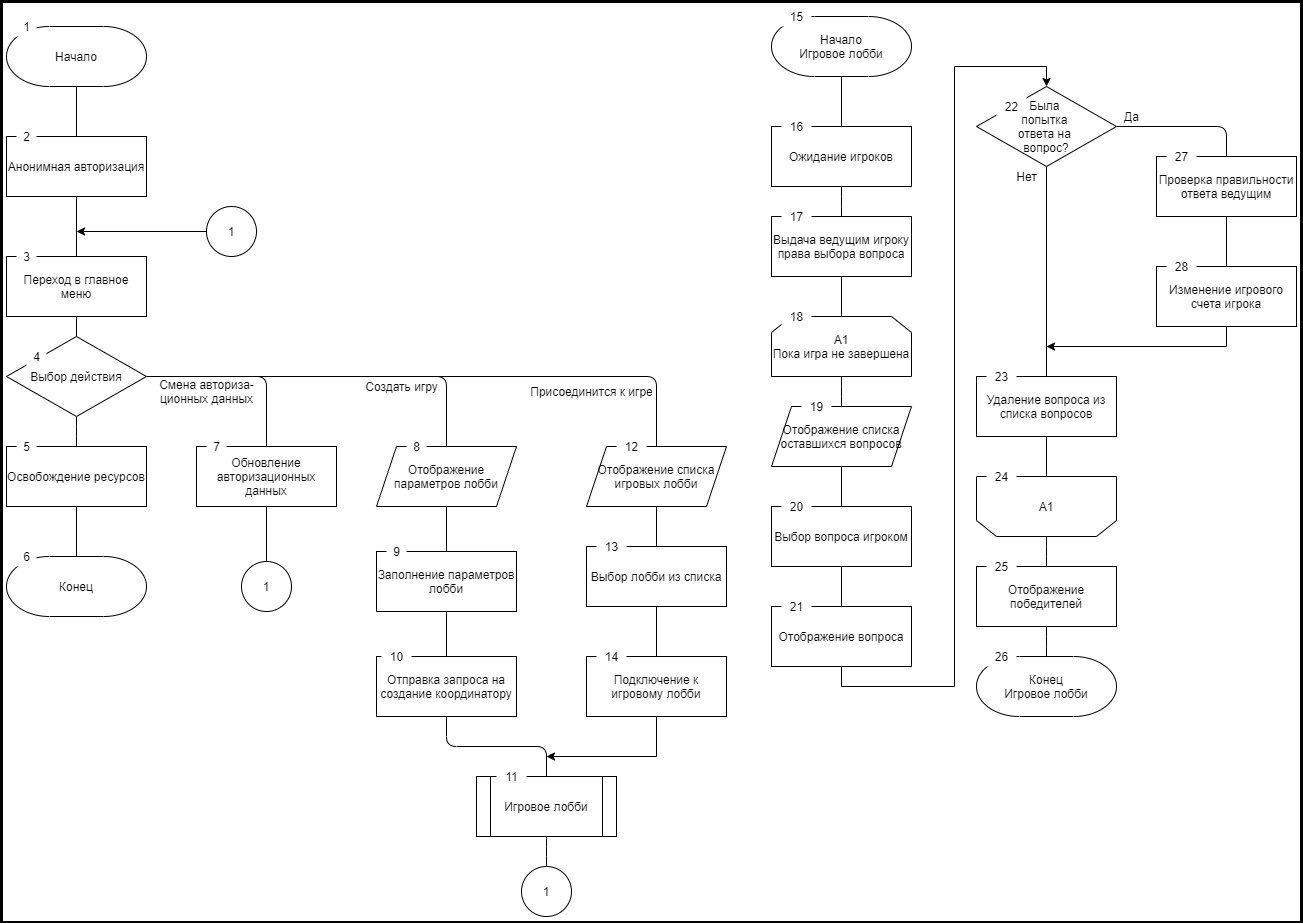
\includegraphics[scale=0.65]{attachments/game_play_alg.png}
	\caption{Схема программы клиентской части программного средства}
	\label{fig:design:client:ux:game_play_alg}
\end{sidewaysfigure}

Таким образом, составленная схема клиентской части программного средства будет использована при разработке непосредственно самого приложения.

\subsubsection{} Конструирование клиентской части приложения
\label{sec:design:client:development}

Наконец, по завершению этапов проектирования и подготовки можно приступить к собственно созданию исходных кодов приложения. Ключевые фрагменты кода, описание которых приведено в данном пункте, приведены в приложении.

Для начала необходимо создать проект типа WPF, с целевой платформой .NET Core \cite{clr_csharp}. Структура проекта будет иметь следующий вид:

\begin{enumerate}
	\item папка views, содержащая описания UI;
	\item папка viewmodels, содержащая модели представления, для привязки на UI;
	\item папка models, содержащая бизнес-логику по обработке данных с UI;
\end{enumerate}

Вся разделяемая логика вынесена в отдельный проект, туда относятся бизнес-сущности и общие методы обработки. Среди команд реализуется RelayCommand<T>, представляющая из себя
универсальную команду, способную работать с параметрами произвольного типа, благодаря шаблонному типу T. Реализуется два варианта команды: с параметром и без, каждый вариант
применяется по ситуации и избавляет от необходимости писать неэффективный код, в случае, если параметр не нужен.

Также реализуются различные расширения разметки, позволяющие более эффективно разрабатывать пользовательский интерфейс и связанную с ним однобразную логику. Такой подход
исключает необходимость дублирования комманд или логики в случае использования одного и того же элемента управления.

Для упрощения процесса оповещения представлений об изменениях в моделях представлений используется сторонняя библиотека Fody.Property-Changed, ее суть заключается в том,
чтобы автоматически добавлять вызов события PropertyChanged для всех публичных свойств, если модель представления реализует интерфейс INotifyPropertyChanged. Ее использование
уменьшает объем кода, необходимы для описания свойств примерно на 80\%, что значительно ускоряет процесс разработки. Для того, чтобы разработчикам не нужно было везде подключать
эту библиотеку было принято решение о вынесении ее в отдельный базовый класс ViewmodelBase.

Таким образом, были разработаны исходные коды клиентской части приложения. 